%% start of file `template.tex'.
%% Copyright 2006-2013 Xavier Danaux (xdanaux@gmail.com).
%
% This work may be distributed and/or modified under the
% conditions of the LaTeX Project Public License version 1.3c,
% available at http://www.latex-project.org/lppl/.


\documentclass[11pt,a4paper,roman]{moderncv}        % possible options include font size ('10pt', '11pt' and '12pt'), paper size ('a4paper', 'letterpaper', 'a5paper', 'legalpaper', 'executivepaper' and 'landscape') and font family ('sans' and 'roman')

% modern themes
\moderncvstyle{banking}                            % style options are 'casual' (default), 'classic', 'oldstyle' and 'banking'


\moderncvcolor{blue}      


% color options 'blue' (default), 'orange', 'green', 'red', 'purple', 'grey' and 'black'
%\renewcommand{\familydefault}{\sfdefault}         % to set the default font; use '\sfdefault' for the default sans serif font, '\rmdefault' for the default roman one, or any tex font name
\nopagenumbers{}                                  % uncomment to suppress automatic page numbering for CVs longer than one page

% character encoding
\usepackage[utf8]{inputenc}
\usepackage{fontawesome5}
\usepackage{tabularx}
\usepackage{ragged2e}
\usepackage[T1]{fontenc}
\usepackage{lmodern}
\usepackage{academicons}
\usepackage{graphicx}
\usepackage{enumitem}

% adjust the page margins
\usepackage[scale=0.88, top=1.2cm, bottom=1.2cm]{geometry}
\usepackage{multicol}
\usepackage{multirow}

\usepackage{import}

% personal data
\name{Neetu Thapliyal}{}
\address{Research Associate}{New Delhi, India}
\photo [55pt] [] {picture}{}

\newcommand*{\customcventry}[7][.1em]{
	\begin{tabular}{@{}l} 
		{\bfseries #4}
	\end{tabular}
	\hfill% move it to the right
	\begin{tabular}{l@{}}
		{\bfseries #5}
	\end{tabular} \\
	\begin{tabular}{@{}l} 
		{\itshape #3}
	\end{tabular}
	\hfill% move it to the right
	\begin{tabular}{l@{}}
		{\itshape #2}
	\end{tabular}
	\ifx&#7&%
	\else{\\%
		\begin{minipage}{\maincolumnwidth}%
			\small#7%
	\end{minipage}}\fi%
	\par\addvspace{#1}}

\newcommand*{\customcvproject}[4][.1em]{
	\begin{tabular}{@{}l} 
		{\bfseries #2}
	\end{tabular}
	\hfill% move it to the right
	\begin{tabular}{l@{}}
		{\itshape #3}
	\end{tabular}
	\ifx&#4
	\else{\\%
		\begin{minipage}{\maincolumnwidth}%
			\small#4%
	\end{minipage}}\fi%
	\par\addvspace{#1}}

\newcommand*{\cvref}[3][.1em]{
	\begin{tabular}{@{}l} 
		{\bfseries #2}
	\end{tabular}
	\ifx&#3
	\else{\\%
		\begin{minipage}{\maincolumnwidth}%
			\small#3%
	\end{minipage}}\fi%
	\par\addvspace{#1}}

\newcommand{\orcid}[1]{\href{https://orcid.org/#1}{\textcolor[HTML]{A6CE39}{\aiOrcid}}}

\setlength{\tabcolsep}{12pt}

%----------------------------------------------------------------------------------
%            content
%----------------------------------------------------------------------------------
\begin{document}
	\makecvtitle
	\vspace*{-28mm}
	
	\begin{center}
		\small
		\renewcommand{\arraystretch}{1.25}
		\setlength{\tabcolsep}{18pt}
		\begin{tabular}{ l l l }
			\faEnvelope\enspace \href{mailto:neetuthap1602@gmail.com}{neetuthap1602@gmail.com}	& \faLinkedin\enspace \href{https://www.linkedin.com/in/neetu-thapliyal-687a1812a/}{in/neetu-thapliyal} & \multirow{3}{*}{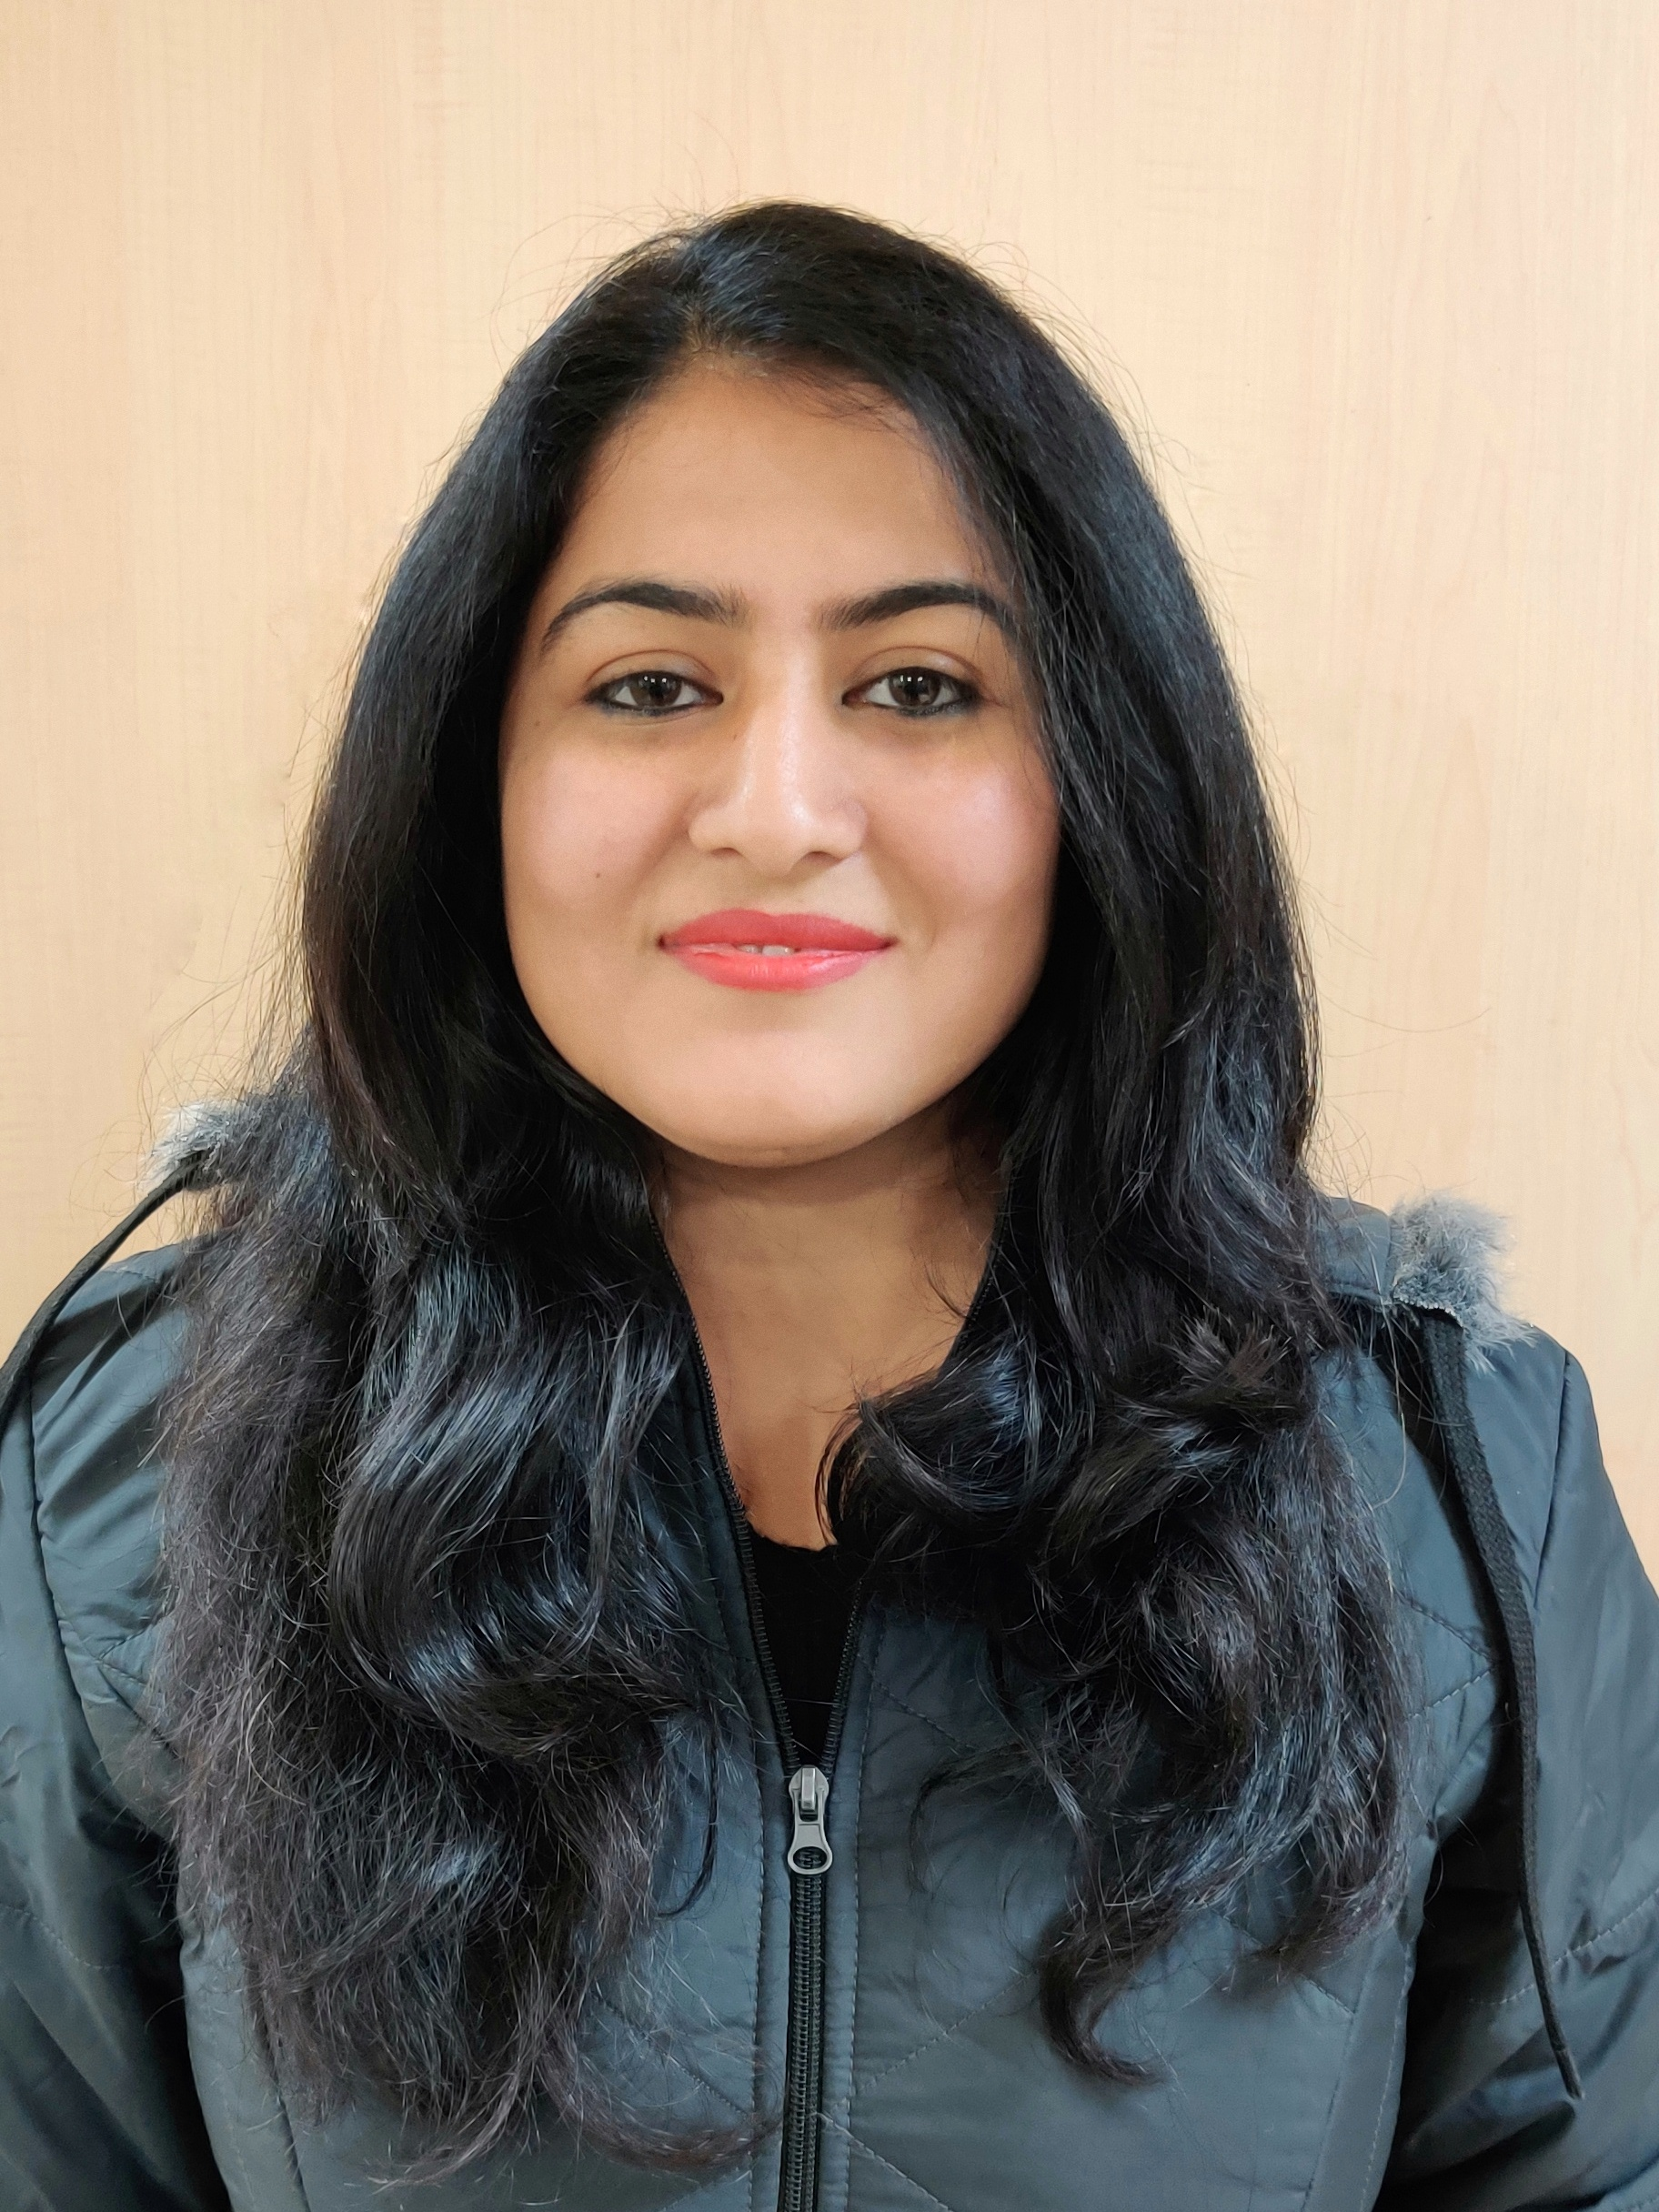
\includegraphics[height=70pt]{picture.jpeg}}\\ 
			\faMobile\enspace +91 7888332014 & \faLink\enspace \href{https://orcid.org/0000-0003-2651-7422}{orcid.org/0000-0003-2651-7422} & \\
			\faMapMarker\enspace New Delhi, India & & \\
		\end{tabular}
	\end{center}
	\vspace*{-4mm}
	
	\section{SUMMARY}
	{Data Analytics professional with 4+ years in market intelligence. Expert in translating complex agricultural and commercial datasets into actionable business strategies and optimized resource models.}

	\section{TECHNICAL SKILLS}
	{\begin{itemize}[noitemsep, topsep=0pt]
			\item \textbf{Analytics:} Statistical Analysis, Trend Identification, Power BI, R, Python, Matlab, Market Research.
			\item \textbf{Expertise:} Competitive Intelligence, Quantitative Research, Stakeholder Management, Report Writing.
		\end{itemize}
	}

	\section{WORK EXPERIENCE}
	
	{\customcventry{May 2020 -- Present}{Lead Analyst}{Mordor Intelligence Private Limited}{Hyderabad, India}{}{}
		{\begin{itemize}[noitemsep, topsep=0pt]
				\item Lead market intelligence research and author comprehensive strategic reports for global clients.
				\item Analyze large-scale datasets and validate insights through C-suite industry stakeholder interactions.
				\item Manage a team of analysts, ensuring high-quality project delivery and commercial research solutions.
		\end{itemize}}
	}

	{\customcventry{Nov 2018 -- May 2020}{Research Associate}{National Seed Association of India (NSAI)}{New Delhi, India}{}{}
		{\begin{itemize}[noitemsep, topsep=0pt]
				\item Managed regulatory and policy matters related to seed legislation and international trade.
				\item Liaised between industry and government bodies to resolve grievances and influence policy frameworks.
		\end{itemize}}
	}

	{\customcventry{Jul 2018 -- Nov 2018}{Junior Research Fellow}{National Agri-Food Biotechnology Institute (NABI)}{Mohali, India}{}{}
		{\begin{itemize}[noitemsep, topsep=0pt]
				\item Conducted advanced research on crop stress tolerance using techniques like SDS-PAGE and HPLC.
		\end{itemize}}
	}

	{\customcventry{Jul 2017 -- Jul 2018}{Assistant Professor}{Lovely Professional University}{Jalandhar, India}{}{}
		{\begin{itemize}[noitemsep, topsep=0pt]
				\item Taught technical courses and developed curricula for agricultural biotechnology training programs.
		\end{itemize}}
	}

	\section{EDUCATION}
	{\customcventry{2015 -- 2017}{M.Sc. Agriculture (Genetics)}{G.B. Pant University}{Pantnagar, India}{}{}{CGPA: 8.55/10.00}}
	{\customcventry{2011 -- 2014}{B.Sc. Lifesciences} {Panjab University}{Chandigarh, India}{}{}{Result: 79\%}}

	\section{AWARDS \& KEY ACHIEVEMENTS}
	{\begin{itemize}[noitemsep, topsep=0pt]
			\item \textbf{Best Thesis Award (2017):} International Conference GRISAAS.
			\item \textbf{GATE Qualified (2017):} 93.7 percentile (AIR 666) in Life Sciences.
			\item \textbf{Scholarship:} Awarded Research Assistantship during Master's (2014--2017).
		\end{itemize}
	} 

	\section{LANGUAGES}
	{English (Fluent), Hindi (Native)}
		
\end{document}
